\begin{mydefs}
	
	\begin{itemize}
		\item Une \kw{droite} est un objet géométrique formé de \kw{points alignés}. 
		\item Une droite est illimitée des deux cotés.
		\item Une droite qui passe par deux points $A$ et $B$, se note $(AB)$ ou $(BA)$;
		\item Si un point $C$ appartient à la droite $(AB)$, on note $C \in (AB)$.
		\item Si il n'appartient pas à la droite $(AB)$, on note $C \notin (AB)$.
	\end{itemize}
\end{mydefs}

\newpage

\begin{myex}
	Les points $M$, $R$ et $A$ sont alignés.
	\begin{center}
		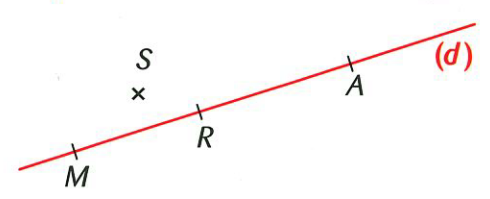
\includegraphics[scale=0.55]{img/droite1}
	\end{center}

	\begin{itemize}
		\item La droite $(d)$ passant par les points $M$ et $R$ se note $(MR)$ ou $(RM)$.
		\item Le point A appartient à la droite $(MR)$, on note : $A \in (MR)$.
		\item Le point S n'appartient pas à la droite $(MR)$, on note : $S \notin (MR)$.
	\end{itemize}
\end{myex}

\begin{mydef}
	\begin{itemize}
		\item Une \kw{demi-droite} est une portion de droite limitée d'un seul côté par un point, son \kw{origine}.
		
		\item La demi-droite d'origine $A$ et passant par $B$ se note% $[AB)$.
	\end{itemize}
	
\end{mydef}


\begin{myex}
	\begin{center}
		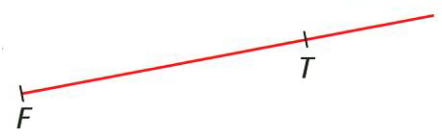
\includegraphics[scale=0.55]{img/demi-droite}
	\end{center}

	 La demi-droite $[FT)$.
\end{myex}

\begin{mydef}
	\begin{itemize}
		\item Un \kw{segment} est une portion de droite limitée par deux points : ses \kw{extrémités}.
		
		\item Le segment d'extrémités $A$ et $B$ se note $[AB]$ ou $[BA]$.
	\end{itemize}
\end{mydef}


\begin{myex}
	\begin{center}
		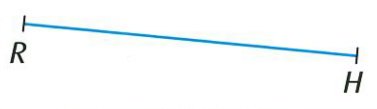
\includegraphics[scale=0.55]{img/segment}
	\end{center}
	
	Le segment $[RH]$ ou $[HR]$.
\end{myex}